
%(BEGIN_QUESTION)
% Copyright 2005, Tony R. Kuphaldt, released under the Creative Commons Attribution License (v 1.0)
% This means you may do almost anything with this work of mine, so long as you give me proper credit

Bestem følgende parametere for disse AC-spenningsformene, forutsatt vertikal følsomhet på 1 volt per rute og tidsbase på 2 millisekunder per rute:

$$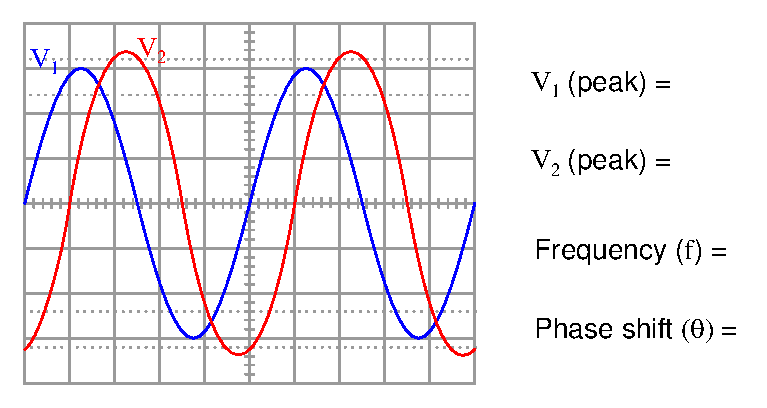
\includegraphics[width=15.5cm]{i00538x01.eps}$$

Bestem også hvilken bølgeform som er \textit{ledende} og hvilken som er \textit{etterslepende}.

\underbar{file i00538}
%(END_QUESTION)





%(BEGIN_ANSWER)

$V_{1}$ (topp) = 3 volt \hskip 100pt $V_{2}$ (topp) = 3.4 volt

\vskip 10pt

$f$ = 100 Hz \hskip 100pt $\theta$ = 72$^{o}$

\vskip 10pt

$V_1$ leder $V_2$ med +72$^{o}$. $V_2$ etterslepper $V_1$ med -72$^{o}$.

%(END_ANSWER)





%(BEGIN_NOTES)

Det er viktig at studentene forklarer \textit{hvordan} de løste faseskiftet, fordi mange har en tendens til å følge en pugget formel, eller enda verre, en annens puggete formel. Dette er et svært enkelt problem å løse, selv om det eneste man husker om en sinusbølge er at en hel periode er 360 grader.

%INDEX% Elektrisitetsrepetisjon: måling av faseskift (dobbeltspors oscilloskop)

%(END_NOTES)

